Una primera idea de solucíon sería para cada pregunta $Q$, simplemente evaluar cada una de las
funciones del conjunto y determinar la que tenga menor valor para el valor $x$ dado. Si $M$ líneas son
dadas junto con $Q$ preguntas, la complejidad de esta solución es O($MQ$). El truco que se presenta a
continuación permite bajar la complejidad a O($(Q+M)\log M$).

Considere la figura  de arriba. Note que la línea $y = 4$ nunca será mínima, independientemente del valor 
de $x$. Del resto de las tres líneas, cada una será la mínima en un solo continuo intervalo (posiblemente 
teniendo más o menos infinito por los límites). Podemos ver que la línea discontinua en verde es la mejor 
para todos los valores de $x$ menores que la intersección con la verde continua más oscura, esta es la mejor
entre esa intersección y su intersección con la verde continua más clara, y esta última es la mejor para
valores de x más grandes. Note también que a medida que $x$ incrementa, la pendiente de la línea mínima
decrece:$\frac{2}{3},-\frac{1}{2},-3$. No es difícil ver que esto siempre ocurre.

Entonces, si eliminamos las líneas irrelevantes, tales como $y = 4$ en este ejemplo (líneas que nunca
darán la mínima y-coordenada, independientemente de la pregunta) y ordenamos el resto de las líneas
por sus pendientes, obtenemos una colección de $N$ intervalos (donde $N$ es el número de líneas restantes),
cada uno perteneciente a una línea en el domino donde es la mínima. Si determinamos los puntos finales
de esos intervalos, utilizando búsqueda binaria se responden cada una de las preguntas.

Como ya hemos visto, si el conjunto de relevantes líneas ha sido determinado y ordenado, es muy
fácil responder las preguntas en O($\log N$) de complejidad usando búsqueda binaria. De esta manera si
nosotros podemos añadir una línea cada vez a nuestra estructura de datos, recalculando esta información
rápidamente con cada adición, tenemos un factible algoritmo: iniciar no con todas las líneas (una o dos
dependiendo de los detalles de la implementación) y añadir líneas una por una hasta que todas las líneas
hayan sido añadidas y nuestra estructura de datos está completa

Supongamos que hemos sido capaz de procesar todas las líneas antes de necesitar la respuesta a
cualquier pregunta. Entonces nosotros podemos ordenarlas descendentemente por pendiente de antemano,
y luego añadirlas una por una. Cuando se añade una nueva línea, algunas líneas pueden ser eliminadas
porque ya no son más relevantes. Si nos imaginamos las líneas en una pila (contiene al elemento más
reciente insertado en el tope de la pila), como añadimos cada nueva línea, consideramos si la línea en el
tope de la pila ya no es relevante; si todavía lo es, insertamos nuestra nueva línea. Sino, sacamos de la
pila la línea del tope y repetimos este procedimiento hasta que la línea del tope sea relevante o quede
solo una línea en la pila

Cómo podemos determinar si la línea debe ser sacada de la pila?

Supongamos que $l_1$, $l_2$ y $l_3$ son la segunda línea del tope, la línea del tope y la línea a añadir
respectivamente. Entonces, $l_2$ se convierte en irrelevante si y solo si el punto de intersección entre $l_1$ y $l_3$ está más a la izquierda que el de la intersección entre $l_1$ y $l_2$. Esto tiene sentido porque significa que el intervalo en el cual $l_3$ abarca es menor que el que abarcaba previamente $l_2$. Supongamos para mayor simplicidad que no hay tres líneas concurrente.

La idea de este enfoque es mantener una envoltura convexo inferior de funciones lineales. En realidad 
sería un poco más conveniente considerarlas no como funciones lineales, sino como puntos $(k;b)$ en el 
plano tal que tendremos que encontrar el punto que tiene el menor producto escalar con un punto dado $(x;1)$, es decir, para este punto $kx+b$ se minimiza, que es lo mismo que el problema inicial. Tal mínimo necesariamente estará en una envoltura convexa más baja de estos puntos como se puede ver a continuación:

\begin{figure}[h!]
	\centering
	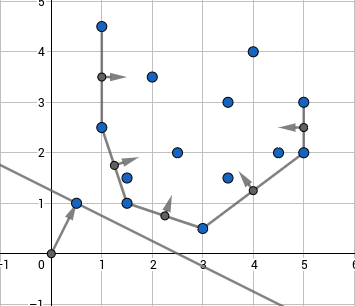
\includegraphics[width=0.2\linewidth]{img/convex_hull_trick2}
	\label{fig:l}
\end{figure}

Uno tiene que mantener puntos en la envoltura convexa y vectores normales de los bordes de la envoltura convexa. Cuando usted tiene una $(x;1)$ consulta tendrás que encontrar el vector normal más cercano a él en términos de ángulos entre ellos, entonces la función lineal óptima corresponderá a uno de sus puntos finales. Para ver eso, se debe notar que los puntos que tienen un producto escalar constante con $(x;1)$ se encuentran en una línea que es ortogonal a $(x;1)$ , por lo que la función lineal óptima será aquella en la que tangente a la envoltura convexa que sea colineal con normal a $(x;1)$ toca la envoltura. Este punto es aquel en el que las normales de las aristas situadas a la izquierda y a la derecha de él están encabezadas en diferentes lados de $(x;1)$. 

